% DarkLens: IEEE conference paper (IEEEtran V1.8b, conference mode, as in IEEE's official template).
% IEEEtran.cls / IEEEtran.bst are included in this folder, so it compiles locally and on Overleaf.
% All numbers come from paper/generated/*.tex, written by scripts/make_paper_assets.py.
\documentclass[conference]{IEEEtran}
\IEEEoverridecommandlockouts
\usepackage{cite}
\usepackage{amsmath,amssymb,amsfonts}
\usepackage{graphicx}
\usepackage{textcomp}
\usepackage{xcolor}
\usepackage{booktabs}
\usepackage{url}
\usepackage{algorithm}
\usepackage{algpseudocode}
\newcommand{\pend}{\textcolor{red}{[pending]}}
\makeatletter\newcommand{\inputtab}[1]{\@@input #1 }\makeatother
% generated by scripts/make_paper_assets.py — do not edit
\newcommand{\LLMmodel}{\pend{}}
\newcommand{\NText}{2356}
\newcommand{\NTextDark}{1178}
\newcommand{\NHeld}{471}
\newcommand{\CVlrF}{0.960}
\newcommand{\CVlrP}{0.968}
\newcommand{\CVlrR}{0.952}
\newcommand{\CVlrMacro}{0.769}
\newcommand{\CVsvmMacro}{0.787}
\newcommand{\CVruleP}{0.995}
\newcommand{\CVruleR}{0.550}
\newcommand{\CVruleF}{0.709}
\newcommand{\LLMtextF}{\pend{}}
\newcommand{\LLMtextMacro}{\pend{}}
\newcommand{\LLMtextSingleMacro}{\pend{}}
\newcommand{\LLMstageOneMacro}{\pend{}}
\newcommand{\LLMstageOneP}{\pend{}}
\newcommand{\LLMtextP}{\pend{}}
\newcommand{\WebOffF}{0.673}
\newcommand{\WebOffP}{0.545}
\newcommand{\WebOffR}{0.880}
\newcommand{\WebOffMacro}{0.339}
\newcommand{\WebLLMF}{\pend{}}
\newcommand{\WebLLMMacro}{\pend{}}
\newcommand{\NWeb}{162}
\newcommand{\TbN}{43}
\newcommand{\TbOffRecall}{100.0\%}
\newcommand{\TbOffPrec}{84.8\%}
\newcommand{\TbOffFP}{9}
\newcommand{\TbOffPrefilter}{45.6\%}
\newcommand{\TbLLMRecall}{\pend{}}
\newcommand{\TbLLMFP}{\pend{}}
\newcommand{\TuneBest}{0.50}
\newcommand{\CrawlAttempted}{\pend{}}
\newcommand{\CrawlOK}{\pend{}}
\newcommand{\CrawlBlocked}{\pend{}}
\newcommand{\CrawlBlockedPct}{\pend{}}
\newcommand{\CrawlOKCountries}{\pend{}}
\newcommand{\CrawlSites}{\pend{}}
\newcommand{\CrawlStates}{\pend{}}
\newcommand{\CrawlAny}{\pend{}}
\newcommand{\CrawlP}{\pend{}}
\newcommand{\CrawlR}{\pend{}}
\newcommand{\CrawlF}{\pend{}}
\newcommand{\CrawlKappa}{\pend{}}
\newcommand{\CrawlNGold}{\pend{}}
\newcommand{\HumanKappa}{\pend{}}


\begin{document}

\title{DarkLens: Auditing EU E-Commerce Websites for Dark Patterns with a Crawl-and-Verify LLM Pipeline}

\author{%
\IEEEauthorblockN{Ashka Jain}
\IEEEauthorblockA{\textit{Dept. of Computer}\\
\textit{Engineering}\\
\textit{Dwarkadas J. Sanghvi}\\
\textit{College of Engineering}\\
Mumbai, India\\
ashkaj79@gmail.com}
\and
\IEEEauthorblockN{Aarya Singh}
\IEEEauthorblockA{\textit{Dept. of Computer}\\
\textit{Engineering}\\
\textit{Dwarkadas J. Sanghvi}\\
\textit{College of Engineering}\\
Mumbai, India\\
aaryadsingh8115@gmail.com}
\and
\IEEEauthorblockN{Devanshi Shah}
\IEEEauthorblockA{\textit{Dept. of Computer}\\
\textit{Engineering}\\
\textit{Dwarkadas J. Sanghvi}\\
\textit{College of Engineering}\\
Mumbai, India\\
askfordevanshi@gmail.com}
\and
\IEEEauthorblockN{Dhruv Patel}
\IEEEauthorblockA{\textit{Dept. of Computer}\\
\textit{Engineering}\\
\textit{Dwarkadas J. Sanghvi}\\
\textit{College of Engineering}\\
Mumbai, India\\
\textcolor{red}{[email]}}
}

\maketitle

\begin{abstract}
Dark patterns---interface designs that push people toward choices they would not otherwise make---are
now a compliance question under the EU Digital Services Act, yet auditing them still depends on manual
inspection of individual pages. We present \emph{DarkLens}, an open pipeline that crawls e-commerce
websites, reaches the product, cart, checkout and cancellation states where dark patterns concentrate
through a safe-interaction policy, represents every visible element together with its UI state, and
classifies it with a cascade of a cheap lexical pre-filter and a large language model (LLM) that first
infers and then verifies each finding. We evaluate on three public datasets, a controlled test-bed of 43
injected patterns with a clean twin site, and a crawl of \CrawlAttempted{} EU retailers, of which
\CrawlOK{} could be crawled and \CrawlBlockedPct{} refused automated browsers; a stratified sample of the crawl was
labelled by two annotators. A grouped cross-validated TF-IDF baseline already reaches F1~=~\CVlrF{} on binary text
detection but only \CVlrMacro{} macro-F1 across categories, and it raises false alarms on neutral text
such as ``In stock'' when the page context is missing. On the test-bed the LLM pipeline finds \TbLLMFound{} of
\TbN{} injected patterns and raises \TbLLMFP{} false alarm on the clean twin, against \TbOffFP{} for the lexical engine. It reaches \LLMtextMacro{} macro-F1
on held-out text, \WebLLMF{} F1 on AidUI web screenshots, and F1~=~\CrawlF{} (Cohen's $\kappa$~=~\CrawlKappa{})
against human ground truth on the live crawl, where \CrawlAny{} of sites show at least one pattern. We
release the crawler, the test-bed, the annotation tool and a web interface that marks dark patterns on an
uploaded screenshot.
\end{abstract}

\begin{IEEEkeywords}
dark patterns, deceptive design, large language models, web crawling, consumer protection, Digital Services Act
\end{IEEEkeywords}

% =====================================================================
\section{Introduction}
Countdown timers that restart on reload, ``only 2 left'' badges, opt-out links worded as ``No thanks,
I prefer paying full price'', protection plans ticked by default in the basket, and memberships that can
only be cancelled by phone are all instances of \emph{dark patterns}~\cite{brignull2010,gray2018}.
Mathur et al.\ found such patterns on 11.1\% of 11{,}000 shopping websites~\cite{mathur2019}, and Nouwens
et al.\ showed that only 11.8\% of consent banners on popular UK sites met the GDPR's minimum
requirements~\cite{nouwens2020}. In the EU, Article~25 of the Digital Services Act (DSA) prohibits online
platforms from designing interfaces that deceive or manipulate users~\cite{dsa2022}, the Unfair Commercial
Practices Directive blacklists false ``very limited time'' claims~\cite{ucpd2005}, and the Consumer
Rights Directive forbids pre-ticked boxes for extra payments~\cite{crd2011}. Regulators therefore need
measurements that are repeatable at scale, not one-off manual reviews.

Automatic detection has advanced from bag-of-words classifiers on extracted text~\cite{yada2022} to
multimodal LLM pipelines on screenshots~\cite{lin2026dpdgpt}. Three gaps remain. First, most detectors are
evaluated on curated snippets or screenshots, not on pages a crawler has to reach---and many patterns only
appear after an interaction (opening a cookie layer, adding to basket). Second, text-only models lose the
UI state that defines several patterns: the words ``Add protection plan'' are harmless unless the box is
ticked. Third, the reliability of LLM judgements against humans on live, messy sites is an open question:
Nwokeji et al.\ report that UX experts recall more dark patterns than vision LLMs on static
screenshots~\cite{nwokeji2026}.

We make the following contributions:
\begin{itemize}
\item \textbf{A priority-guided crawler with a safe-interaction policy} that reaches cart, checkout and
cancellation states on any shop, opens cookie layers and pop-ups, never pays or submits personal data,
and records HTML, text, screenshots and every UI element with its geometry, style and checked state.
\item \textbf{A state-aware segment representation and cascade detector}: elements are serialised with their
UI state (e.g.\ ``[checkbox, PRE-TICKED]''), filtered by a rule lexicon and TF-IDF classifier, then labelled
by an LLM in an infer stage and re-checked in a verify stage adapted from DPDGPT~\cite{lin2026dpdgpt}.
The same detector serves screenshots through OCR-anchored prompting, so every finding has a location.
\item \textbf{A three-level evaluation}: public datasets (text and screenshots), a controlled test-bed with
known ground truth and a clean twin, and an EU crawl with double human annotation, including a measurement of how
many retailers block automated auditing at all.
\item \textbf{An open tool}: a web interface that analyses an uploaded screenshot or a live URL and shows
the category, evidence, confidence and the EU provision an auditor would examine.
\end{itemize}

% =====================================================================
\section{Related Work}
\textbf{Measurement studies.} Mathur et al.\ crawled 11K shopping sites, segmented pages into text blocks,
clustered them and labelled 1{,}818 instances in 15 types and 7 categories~\cite{mathur2019}; their
taxonomy and data underpin most later work, including ours. Nouwens et al.\ scraped consent
management platforms and measured how interface design changes consent rates~\cite{nouwens2020}. Di
Geronimo et al.\ found dark patterns in 95\% of 240 popular mobile apps~\cite{digeronimo2020}.

\textbf{Text classification.} Yada et al.\ turned Mathur's strings into a balanced binary dataset with
non-dark text from the same sites and reported F1~=~0.960 for logistic regression and 0.975 for
RoBERTa-large~\cite{yada2022}; a follow-up adds post-hoc explanations~\cite{yada2024}. These models see
isolated snippets without page context or UI state.

\textbf{Multimodal and LLM detection.} AidUI combines object detection and NLP on screenshots and reaches
precision 0.66, recall 0.67 and F1 0.65 over ten pattern types on its ContextDP dataset~\cite{mansur2023}.
DPDGPT prompts a multimodal LLM through extraction, initial inference, verification and advanced
inference and reports precision 0.86, recall 0.91 and F1 0.88 across 19 types on
ContextRico-DP~\cite{lin2026dpdgpt}. Nwokeji et al.\ compare UX experts with vision LLMs in an
asymmetric design (experts rate GPT-4.1-generated interfaces, LLMs rate human-made ContextDP screenshots)
and find that experts achieve higher recall~\cite{nwokeji2026}. DarkBench evaluates manipulative
behaviour of chatbots themselves and validates an LLM judge against humans~\cite{kran2025darkbench}.

\textbf{Dark patterns and agents.} LLM web agents fall for a single dark pattern about 41\% of the time
in the TrickyArena environment~\cite{ersoy2026}, and GUI agents often fail to recognise manipulative
interfaces even when humans oversee them~\cite{tang2025gui}. As agents shop on users' behalf, auditing
interfaces becomes more pressing.

\textbf{Regulation.} Ahuja et al.\ map 59 dark patterns to the DSA's notions of deception, manipulation
and impairment of autonomy and show that context decides whether a pattern is a violation~\cite{ahuja2026dsa}.
We therefore report legal provisions as pointers for an auditor, not as verdicts.

DarkLens differs from these systems by detecting on states the crawler reaches itself, by encoding UI state
into the model input, and by measuring reliability against humans on a live EU crawl.

% =====================================================================
\section{The DarkLens Pipeline}
Fig.~\ref{fig:arch} shows the six stages.

\begin{figure*}[t]
\centering
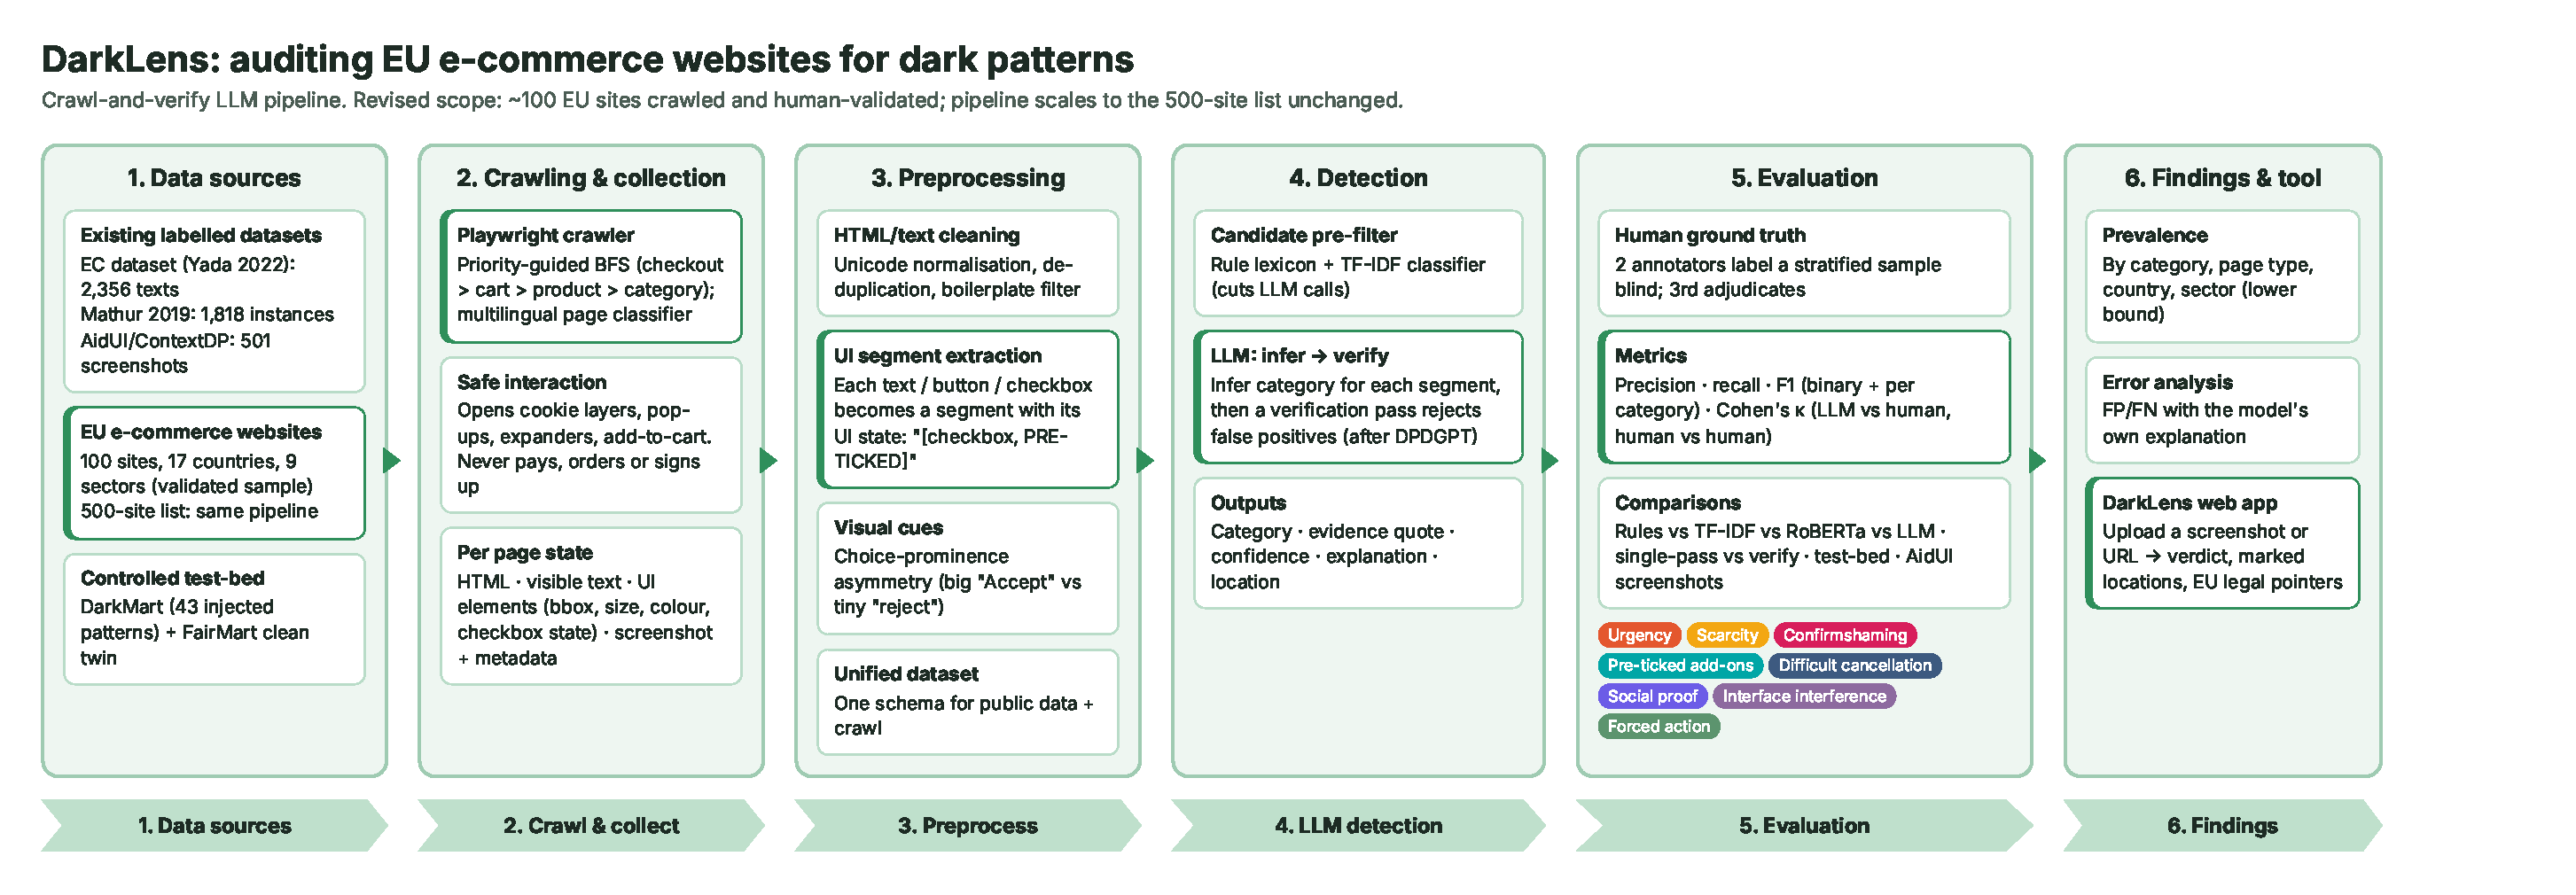
\includegraphics[width=\textwidth]{generated/fig_architecture.pdf}
\caption{DarkLens architecture. Public datasets and a controlled test-bed calibrate and benchmark the
detector; the crawler collects live EU pages; human annotation provides ground truth for evaluation.}
\label{fig:arch}
\end{figure*}

\subsection{Taxonomy}
We keep five core classes from our project scope---urgency, scarcity, confirmshaming, pre-ticked
add-ons/sneaking and difficult cancellation (obstruction)---and add social proof, interface interference and
forced action, which are frequent in the public data and in screenshots. Table~\ref{tab:tax} maps each
class to Mathur et al.'s types~\cite{mathur2019} so results remain comparable.

\begin{table}[t]
\centering
\caption{DarkLens taxonomy and its mapping to Mathur et al.~\cite{mathur2019}.}
\label{tab:tax}
\footnotesize
\begin{tabular}{p{2.1cm}p{5.6cm}}
\toprule
Class & Mathur et al.\ types (category) \\
\midrule
Urgency & Countdown timer; limited-time message (Urgency) \\
Scarcity & Low-stock; high-demand message (Scarcity) \\
Social proof & Activity notification; testimonials of uncertain origin \\
Confirmshaming & Confirmshaming (Misdirection) \\
Pre-ticked add-ons / sneaking & Sneak into basket; hidden costs; hidden subscription; pressured selling \\
Difficult cancellation & Hard to cancel (Obstruction) \\
Interface interference & Visual interference; trick questions (Misdirection) \\
Forced action & Forced enrollment (Forced Action) \\
\bottomrule
\end{tabular}
\end{table}

\subsection{Priority-guided crawler with safe interaction}
The crawler (Playwright, Chromium) keeps a max-heap of URLs keyed by a relevance score
(Algorithm~\ref{alg:crawl}). A multilingual page classifier assigns a type from URL tokens, title and
content (an add-to-cart button with few prices indicates a product page); base scores rank checkout (10)
$>$ cart, subscription (9) $>$ product (8) $>$ category (5) $>$ homepage (3) $>$ informational pages (0),
with bonuses for anchor text such as ``basket'' or ``zur Kasse'' and a small depth penalty. Keyword lists
cover nine EU languages.

On each page the crawler tries up to three \emph{safe interactions}, chosen by type: opening cookie
settings, dismissing pop-ups through their decline option, expanding details, choosing variants and---when
enabled, as in~\cite{mathur2019}---adding one product to the basket so that cart and checkout states exist.
A three-tier policy blocks anything that pays, places an order, signs up, submits data, deletes or logs
out, in nine languages. Each resulting state is captured as rendered HTML, visible text, a full-page
screenshot and a list of UI elements with bounding box, font size and weight, colours, overlay membership
and, for form controls, the checked or selected value. The crawler respects \texttt{robots.txt}, waits
between requests and stops after a page and time budget per site.

\begin{algorithm}[t]
\caption{Priority-guided crawl with safe interaction}
\label{alg:crawl}
\footnotesize
\begin{algorithmic}[1]
\State $Q \gets \{(\mathrm{score}(s_0), s_0, 0)\}$, $V \gets \emptyset$
\While{$Q \neq \emptyset$ \textbf{and} $|V| < N_{\max}$ \textbf{and} time $<$ budget}
  \State $(\cdot, u, d) \gets \mathrm{pop\_max}(Q)$; \textbf{skip} if $u \in V$, $d > D_{\max}$ or robots disallow
  \State load $u$; $S \gets \mathrm{capture}(u)$; $t \gets \mathrm{classify}(u, S)$; $V \gets V \cup \{u\}$
  \ForAll{same-site links $(v, a)$ in $S$}
    \State push $(\mathrm{base}(t_v) + \mathrm{anchor}(a) - 0.25(d{+}1), v, d{+}1)$ to $Q$
  \EndFor
  \ForAll{$e \in \mathrm{top}_k(\mathrm{revealing\ elements\ of\ } S)$ with $\mathrm{tier}(e) \neq$ blocked}
    \State click $e$; $S' \gets \mathrm{capture}$; store $(S, e, S', \Delta)$; enqueue new links
  \EndFor
\EndWhile
\end{algorithmic}
\end{algorithm}

\subsection{State-aware segments}
Preprocessing turns each state into \emph{segments}: visible text blocks, buttons, links, checkboxes,
radio buttons and drop-downs, after Unicode normalisation, de-duplication and removal of navigation
labels and bare prices. Text that labels a form control is folded into the control. Each segment carries
a short UI descriptor, so the model reads ``[checkbox, PRE-TICKED] Add 2-year protection plan
(+\texteuro19.99)'' rather than the bare words. A geometric check also emits a \emph{choice pair} segment when
two nearby controls in a pop-up or on a decision page differ in area by $\geq 3\times$ or in font size by
$\geq 1.6\times$---the visual signature of interface interference.

\subsection{Cascade detection: pre-filter, infer, verify}
\textbf{Pre-filter.} A rule lexicon (regular expressions per class in six languages) and a TF-IDF logistic
regression keep a segment if a rule fires, if $p(\text{dark}) \geq 0.2$, or if it is a pre-ticked control, a
drop-down or a choice pair. On the EC held-out split this threshold keeps 98.3\% of dark items while forwarding
8.9\% of non-dark ones (0.15 would keep 98.7\% but forward 14.5\%); everything else is labelled not dark without
an LLM call, and the annotated crawl sample measures what the pre-filter misses in practice.

\textbf{Infer.} Elements that repeat across a shop's pages---cookie banner, menu, footer, newsletter
pop-up---are classified once per site and the answer is applied to every occurrence, so the LLM sees each
distinct element exactly once (on the test-bed this removes 73\% of LLM inputs). Each element is tagged with the
type of page it first appeared on and sent in order of first appearance, in batches of up to 80, together with
the site's country and language, the taxonomy definitions with counter-examples, and few-shot examples drawn only
from the training split. The model returns, per element, a label, a confidence, a verbatim evidence quote and a
one-sentence explanation as JSON.

\textbf{Verify.} Every positive goes to a second call that restates the relevant definitions and
counter-examples and asks the model to keep or reject each candidate and to correct its category; this
mirrors the verification stage that DPDGPT credits for precision~\cite{lin2026dpdgpt}. Running only the
infer stage gives the single-pass ablation.

\textbf{Screenshots.} For an uploaded image, Tesseract~\cite{smith2007tesseract} reads text lines after
$2\times$ up-scaling and adaptive thresholding (needed for text under dimmed pop-up overlays). The image
and the numbered OCR lines go to a vision LLM, which cites line identifiers for textual patterns and gives
approximate boxes for purely visual ones; detections are then verified as above. Line identifiers ground
each finding to pixel coordinates regardless of the LLM's own localisation ability. Tall pages are tiled.

\textbf{Engines.} The LLM client calls Gemini, OpenAI, Anthropic or a local Ollama model through plain
HTTPS, caches every response keyed by model, prompt and image, and logs the model identifier and date.
Without an API key, an \emph{offline engine} replaces the LLM with rules, the TF-IDF model and UI-state
rules (pre-ticked paid/consent options, surcharged default options, choice pairs).

\subsection{Interface}
A FastAPI service and a browser front end let a user drop a screenshot or paste a URL. The result shows a
verdict, numbered boxes on the image linked to a list of findings with category, evidence, confidence,
explanation and the EU provision to examine, and a downloadable JSON report. The same application hosts
the annotation tool used for ground truth (Section~\ref{sec:annot}).

% =====================================================================
\section{Experimental Setup}
\subsection{Data}
\textbf{Text.} The EC dataset~\cite{yada2022} has \NText{} snippets (\NTextDark{} dark, Mathur-derived;
the rest non-dark text from the same sites). We recover Mathur's fine-grained type for every dark snippet
by exact string match, mapping each to our taxonomy. All text models use 5-fold
\emph{StratifiedGroupKFold} grouped by source page, so no page contributes to both training and testing;
one fold (\NHeld{} items) is the fixed held-out split for the LLM, RoBERTa~\cite{liu2019roberta} and
baselines.

\textbf{Screenshots.} AidUI's evaluation set~\cite{mansur2023} has 162 web and 339 mobile screenshots with
localised labels. We tune the only free parameter of the offline engine (the classifier threshold for OCR
lines) on the mobile split, choosing \TuneBest{}, and report on the untouched web split
(\NWeb{} images). Scoring is image-level and multi-label.

\textbf{Test-bed.} \emph{DarkMart} is a local seven-page-type shop with \TbN{} injected instances across all
eight classes (timers, low-stock badges, activity toasts, a confirmshaming newsletter pop-up, pre-ticked
basket add-ons, a surcharged default variant, a hidden checkout fee, forced account creation,
phone-only cancellation, and an asymmetric cookie banner with a pre-ticked consent layer).
\emph{FairMart} has the same structure and copy with every manipulative element removed. We crawl both and
measure instance recall on DarkMart and false alarms on FairMart.

\textbf{EU crawl.} We attempted \CrawlAttempted{} retailers from EU member states across electronics,
fashion, marketplaces, general merchandise, beauty, home, books, grocery, sports and travel, with at most 15
pages and 3 interactions per page. A site counts as \emph{crawlable} if at least two pages loaded; a site whose
first response is a bot-protection or maintenance page (Cloudflare challenge, ``Access Denied'', captcha) is
recorded as \emph{blocked} and not crawled further. We do not attempt to circumvent such protection.
\CrawlOK{} sites in \CrawlOKCountries{} countries were crawlable, and prevalence is computed over these only, so a
block page is never counted as a site without dark patterns.

\subsection{Ground truth and metrics}\label{sec:annot}
We sample 150 crawled page states stratified by page type (at most four per site). Two annotators label
every segment that reached the detector plus a random 15\% of filtered-out segments (to measure pre-filter
misses), independently and blind to model output, using the annotation tool. A third annotator
adjudicates disagreements. We report Cohen's $\kappa$~\cite{cohen1960} between annotators and between
the LLM and the adjudicated labels, Fleiss' $\kappa$~\cite{fleiss1971} when more annotators overlap,
interpreted with Landis and Koch~\cite{landis1977}, and precision, recall and F1, binary and per class
(macro-averaged over dark classes), with 95\% bootstrap intervals.

\subsection{Models}
The LLM is \LLMmodel{} at temperature 0. RoBERTa-base is fine-tuned for four epochs (learning rate
$2{\times}10^{-5}$, batch 32, max length 64) on the same training split.

% =====================================================================
\section{Results}
\subsection{Text detection}
Table~\ref{tab:text} lists all text results. The rule lexicon is precise (\CVruleP{}) but recalls only
\CVruleR{}: dark-pattern copy is too varied for fixed phrasing. TF-IDF with logistic regression reaches
binary F1~=~\CVlrF{} under grouped cross-validation, matching the 0.960 Yada et al.\ report for the same model
on a random split~\cite{yada2022}. The harder question is \emph{which} pattern: macro-F1 across classes is
\CVlrMacro{} (SVM \CVsvmMacro{}), and Fig.~\ref{fig:percat} shows the drop on rare classes---pre-ticked
add-ons, difficult cancellation and interface interference---whose wording overlaps with ordinary checkout
copy. The LLM pipeline reaches \LLMtextMacro{} macro-F1; verification changes binary precision from
\LLMstageOneP{} to \LLMtextP{}.

\begin{table}[t]
\centering
\caption{Text detection on the EC dataset. P/R/F1: binary (dark vs.\ not). Macro-F1: over dark classes.
$^\dagger$Single pass: the infer stage alone, without verification.}
\label{tab:text}
\footnotesize
\begin{tabular}{lcccc}
\toprule
Model & P & R & F1 & Macro-F1 \\
\midrule
\inputtab{generated/tab_text.tex}
\bottomrule
\end{tabular}
\end{table}

\begin{figure}[t]
\centering
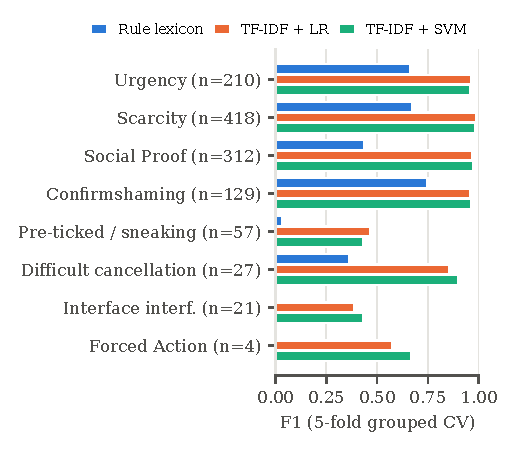
\includegraphics[width=\columnwidth]{generated/fig_percategory.pdf}
\caption{Per-class F1 of the text baselines (5-fold grouped CV). Rare classes are where lexical models fail.}
\label{fig:percat}
\end{figure}

\subsection{Screenshot detection}
Table~\ref{tab:screens} reports image-level results on AidUI web screenshots. The offline engine reads only
text and therefore misses visual patterns (pre-selected options, attention distraction) and short or stylised
copy that OCR damages; it reaches F1~=~\WebOffF{} (precision \WebOffP{}, recall \WebOffR{}). Given only the
image, the vision LLM already reaches F1~=~\WebVisF{} (precision \WebVisP{}, recall \WebVisR{}) and raises
category macro-F1 from \WebOffMacro{} to \WebVisMacro{}. Adding the numbered OCR lines to the prompt, which is
how DarkLens localises findings, gives F1~=~\WebLLMF{}. AidUI's own instance-level scores (F1
0.65~\cite{mansur2023}) use a different unit and are not directly comparable.

\begin{table}[t]
\centering
\caption{Screenshot detection on AidUI web (\NWeb{} images). P/R/F1: does the image contain a dark pattern;
Macro-F1: per category over AidUI's labelled classes.}
\label{tab:screens}
\footnotesize
\setlength{\tabcolsep}{4pt}
\begin{tabular}{lcccc}
\toprule
Engine & P & R & F1 & Macro-F1 \\
\midrule
\inputtab{generated/tab_screens.tex}
\bottomrule
\end{tabular}
\end{table}

\subsection{Controlled test-bed}
The crawler reached all seven page types on both shops, including basket, checkout and the
cancellation page, without a site-specific rule. Table~\ref{tab:testbed} shows that the offline engine finds
\TbOffRecall{} of the \TbN{} injected instances on DarkMart (the UI-state rules recover all pre-ticked
boxes and the surcharged default variant, which text alone cannot), with \TbOffPrec{} of its positive
predictions matching an injected instance. On FairMart it raises \TbOffFP{} false alarms, all from the TF-IDF
model reading neutral words out of context: ``In stock'' (scarcity), ``Cancel membership''
(difficult cancellation) and ``Save'' (pre-ticked add-on). These are exactly the context errors the LLM
stage is meant to remove, and it largely does: with the LLM, DarkLens finds \TbLLMFound{} of the \TbN{} instances
and raises \TbLLMFP{} false alarm on FairMart, reading the neutral ``Keep membership'' button on its cancellation page as
difficult cancellation. Its two misses are the \texteuro4.95 ``service \& handling'' fee that appears only at
checkout---a hidden cost that reads as an ordinary price line unless one knows it was absent from the basket---and
DarkMart's oversized ``Keep my benefits'' button, a visual asymmetry the text pipeline can only describe in words.
Presenting elements page by page instead of once per site found 42 of 43 instances with no false alarm, but needed
about ten times as many LLM calls; we use per-site de-duplication because it makes a 100-site crawl feasible on a
free API tier. The pre-filter sent \TbOffPrefilter{} fewer segments to the detector. Because we
designed the test-bed while developing the rules, it validates function rather than measuring
generalisation.

\begin{table}[t]
\centering
\caption{Controlled test-bed: \TbN{} injected instances on DarkMart; false alarms counted on FairMart
(distinct page/text pairs).}
\label{tab:testbed}
\footnotesize
\setlength{\tabcolsep}{4pt}
\begin{tabular}{lccc}
\toprule
Engine & Recall & Precision & Clean-shop FPs \\
\midrule
\inputtab{generated/tab_testbed.tex}
\bottomrule
\end{tabular}
\end{table}

\subsection{EU crawl: reliability and prevalence}
Annotators agreed with Cohen's $\kappa$~=~\HumanKappa{} on category labels. Against the adjudicated
labels (\CrawlNGold{} segments), DarkLens achieves precision \CrawlP{}, recall \CrawlR{} and F1 \CrawlF{}
(Cohen's $\kappa$~=~\CrawlKappa{}). Across \CrawlSites{} sites and \CrawlStates{} page states, \CrawlAny{}
of sites show at least one pattern; Table~\ref{tab:prev} breaks this down by class. Because LLMs
under-recall relative to people~\cite{nwokeji2026} and the crawler cannot reach log-in-gated flows, these
are lower bounds.

\begin{table}[t]
\centering
\caption{Share of crawled EU sites with at least one detected instance (lower bound).}
\label{tab:prev}
\footnotesize
\begin{tabular}{lc}
\toprule
Class & Sites \\
\midrule
\inputtab{generated/tab_prevalence.tex}
\bottomrule
\end{tabular}
\end{table}

% =====================================================================
\section{Discussion}
\textbf{Context and state matter more than wording.} The strongest lexical model is accurate on curated
snippets, yet on a realistic page it flags ``In stock'' and ``Cancel membership''. Conversely, the most
legally clear-cut pattern in our taxonomy---a pre-ticked paid add-on, prohibited by Article~22 of the
Consumer Rights Directive~\cite{crd2011}---is invisible in text and trivial once the checkbox state is part
of the input. Encoding UI state is cheap and should be standard for detectors that work on crawled pages.

\textbf{Reaching the pattern is half the problem.} Cookie layers, basket add-ons and cancellation flows only
exist after interaction. A priority-guided crawler with an explicit safe-interaction policy gets there
without placing orders, but subscription cancellation behind a log-in remains out of reach without test
accounts. More fundamentally, \CrawlBlockedPct{} of the retailers we attempted---disproportionately the
largest---answered an automated browser with bot protection. Independent auditing of the very platforms with
the most users therefore depends on regulated data access, such as the vetted-researcher provisions of the
DSA~\cite{dsa2022}, rather than on crawling alone, and prevalence estimates from crawls are biased toward smaller
sites that do not deploy such protection.

\textbf{Explanations support auditing.} Each finding carries a quote, a reason and a provision, which made
annotation disagreements and model errors fast to review. Legal pointers are deliberately framed as a
starting point: whether a given banner violates the DSA depends on context~\cite{ahuja2026dsa}.

\textbf{Limitations.} Results depend on the LLM version, which we log; prompts were written in English for
multilingual pages; the site sample over-represents electronics retailers and, because of bot protection,
under-represents the largest platforms; OCR limits the offline
screenshot engine; and the test-bed was built by the authors. Two annotators from the project team are not
domain experts, which we mitigate with written guidelines and adjudication.

\textbf{Ethics.} We crawl only public pages, respect \texttt{robots.txt}, rate-limit requests, never create
accounts, pay or submit personal data, and release no personal data.

% =====================================================================
\section{Conclusion}
DarkLens shows that a crawl-and-verify pipeline, which reaches interaction-dependent states and feeds an LLM
state-aware segments, can audit live EU shops with measured reliability against human labels. The same
pipeline runs unchanged on the full 500-site list; next steps are test accounts for cancellation flows,
evaluation on ContextRico-DP~\cite{lin2026dpdgpt}, and per-language analysis across more EU languages.

\bibliographystyle{IEEEtran}
\bibliography{refs}

\end{document}
